\section{Scalability in the system}
\paragraph{Scalability principles}
In \autoref{sec:scalability} we determined that there are different types of scalability, and that when designing for scalability certain principles should be followed.
In this section we will examine and discuss which of these principles we followed throughout the creation of the system.

\begin{itemize}
    \item \textbf{Design two of everything}: When designing two of everything it is important to identify if there is any single point of failure.
    In our case that would be the API and the database.
    For our API we could start multiple machines that each run an API so that if one fails the others will take over the workload.
    The same would work for the database, but in that case it would need to handle updating the data of each database instance to ensure consistency.
    \item \textbf{Scale horizontally}: Horizontal scaling is the smarter way to scale an application, as we talked about in \autoref{sec:scalability}.
    However, we were only able to test it with vertical scaling as running horizontal scaling required us to run the system on multiple machines and then route the traffic to the different machines.
    We had difficulties in doing this as we were not able to do this on the university network since each machine gets its own subnetwork.
    \item \textbf{Build API first}: Whenever we implemented a new functionality we always started by creating the API endpoints.
    We did this to ensure that the API could be used for other systems in the future and made sure that the data was as generic as possible to not tailor the API for the front end. 
    \item \textbf{Caching data}: Caching data after retrieval could help increase performance of the system if a user were to quickly swap between separate pages. 
    As it stands, our system does not take advantage of caching.
    \item \textbf{Eventual consistency}: The system does not have any parts that strictly require consistency, meaning scalability through availability should be possible. 
    If a user is browsing the services, it is not imperative that, if a new service were to be added, it would update the page the user was using.
    It would simply update the next time the user performed an action to change the state of the system, at which point the new data would be loaded and shown.
    \item \textbf{Easy maintenance and automation}: In order to make maintenance easy, the system has been designed to split responsibility.
    If an update to the system was necessary, we attempted to make it easy by ensuring it would not require changes in multiple files.
    \item \textbf{Write asynchronous code}: Allowing tasks to be executed on different threads is a way to increase availability. 
    This was a primary concern when implementing the system, and all interactions between the API and the database, and the front end and API are processed asynchronously.
    If the code would not have been asynchronous it would have meant enormous idle times where the program would have waited for I/O actions to return.
    \item \textbf{Storing information in the state}: The system does not store information about a component's state in the system servers.
    As part of using React, the system stores information about states on the client side.
    This means that any server can handle any client request, and they will not depend on each other.
\end{itemize}
We attempted to keep many of these design principles in mind when creating the system to increase scalability.
However, we did not fully manage to account for all of them.
A principle such as caching data would be beneficial, and is an obvious point of improvement for the system.
Another point of improvement could be introducing pagination on some of the components that would benefit from it, to ensure the amount of data does not scale to be unnecessarily large.

\paragraph{Deployment architecture}
If the system were to be deployed, the diagram of components would be as illustrated in \autoref{fig:deployment-diagram}.
\begin{figure}[H]
    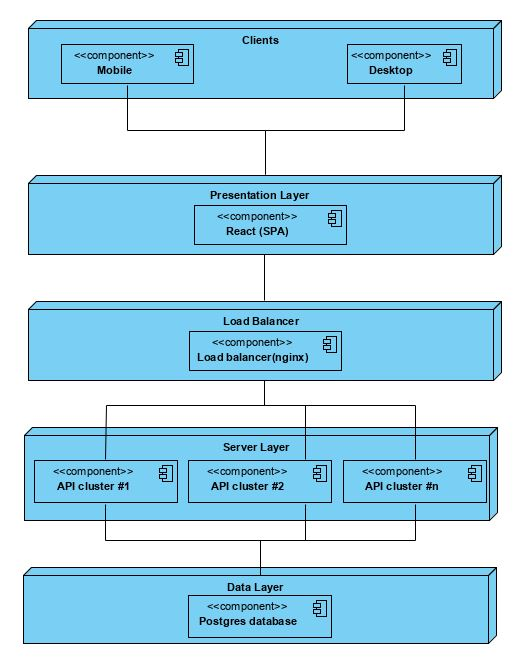
\includegraphics[height=15cm]{/deployment.JPG}
     \caption{The deployment diagram for the system}
     \label{fig:deployment-diagram}
 \end{figure}
 \noindent
As shown, this would involve a horizontal scaling, with the main changes happening in the load balancer and server layer.
The load balancer would be responsible for distributing clients to different API clusters.
While there are different API cluster in order to spread out client requests, each cluster would also have multiple instances of the API, meaning an API cluster could consists of one to many API's.

\subsection{Evaluation of API scalability}
To evaluate the scalability in terms of availability, we ran load tests to test whether using a vertical scaling model worked.
As most of the business logic is handled by the API, it was decided to focus load test on the API.
We decided to do a peak load test using the tool \texttt{LoadUI}, which allows us to define an amount of arriving virtual users (VUs) \cite{loadimpactSource}. 
These VUs work as concurrent users that were each can open multiple connections in parallel to simulate having a large amount of users constantly arriving to the site.
Unlike real users, these VUs will continuously send requests to the server at a rate of approximately 18 requests per second, as seen on the results in the appendix\autoref{App:LoadTestResults}.
\\
For the load tests we used a setup where 20 new VUs would arrive every 10th second, and a test duration of five minutes.
The tests were ran with the following vertical scaling setups:
\begin{itemize}
    \item 1 cluster with 1 instance
    \item 1 cluster with 1 instance
    \item 1 cluster with 8 instances
    \item 1 cluster with 16 instances
    \item 1 cluster with 32 instances
\end{itemize}
For all the tests, the API clusters were run on a Lenovo Legion Y530 laptop, using PM2 which is a process manager for Node.js which was responsible for handling the vertical scaling\cite{PM2}.

\begin{table}[]
    \begin{tabular}{|l|l|l|l|l|l|}
    \hline
    \textbf{Amount of instances} & \textbf{1} & \textbf{4} & \textbf{8} & \textbf{16} & \textbf{32} \\ \hline
    Shortest response time       & 29 ms      & 13 ms      & 19 ms      & 27 ms       & 55 ms       \\ \hline
    Longest response time        & 3451 ms    & 2609 ms    & 2509 ms    & 2387 ms     & 12182 ms    \\ \hline
    Average response time        & 771 ms     & 633 ms     & 593 ms     & 582 ms      & 657 ms      \\ \hline
    Failed assertions \%         & 20\%       & 9\%        & 9\%        & 6\%         & 8\%         \\ \hline
    \end{tabular}
    \caption{Summary of load test results.}
    \label{table:load-test-table}
\end{table}

For all tests, we asserted that endpoints should respond within 800 ms, or it should be tagged as failed.
As seen on \autoref{table:load-test-table}, the amount of failed assertions decreased as the cluster size increased, up until 32 instances, where the response times started increasing.
\\
We deem that, even though the amount of VUs is relatively low, the system should be able to sustain a significantly higher amount of real users, as they would most likely not be sending constant requests in the same manner that the VUs do.
In general, we estimate that the average user would send less than one request per second on average, meaning that it is less than 18 times the load the VUs subjected the API to.
\\
This means that we, in theory, should be able to support at least 20*18=360 arriving users every 10th second with this current setup.
For a real deployment of the service, the clusters would probably be split between multiple servers for horizontal scaling, and more specialized hardware that allows for better vertical scaling.
